\documentclass{beamer}

\usetheme{Boadilla}
\beamertemplatenavigationsymbolsempty

\usepackage{graphicx}
\usepackage{subcaption}

\title{docmgr Overview}
\subtitle{Word index manager for documents}
\author[Facundo E. \and Iñaki R.]{Facundo Escobar \and Iñaki Rodriguez}
\institute[UnCuyo]{Universidad Nacional de Cuyo}
\date{\today}

\begin{document}

\begin{frame}
  \titlepage
\end{frame}

\begin{frame}[c]
  \frametitle{Command line syntax}
  \centering
  \texttt{docmgr [options] [file1 file2 ...]}
\end{frame}

\begin{frame}
  \frametitle{Data structure}
  \begin{figure}
    \includegraphics[width=0.3\linewidth]{structure.png}
    \caption{High level description of the software data structure.}
    \label{fig:structure1}
  \end{figure}
\end{frame}

\begin{frame}[c]
  \frametitle{Trie implementation}
  \centering
  The indexing trie consists in lists for the children of each node instead of arrays or
  binary trees.
\end{frame}

\begin{frame}
  \frametitle{Hashmap implementation}
  \begin{figure}
    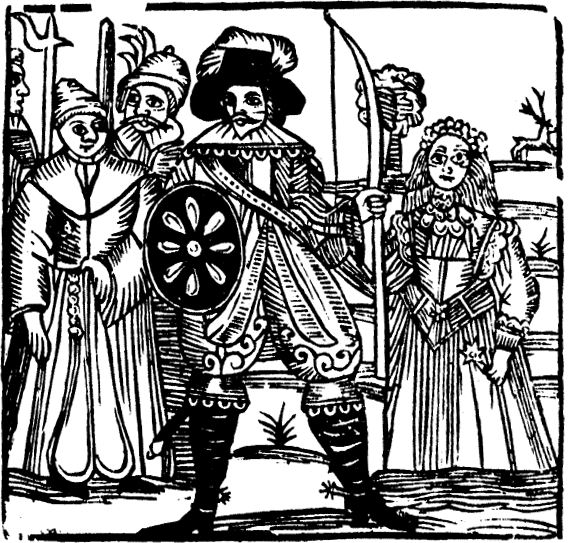
\includegraphics[width=0.3\linewidth]{Robin-hood-and-maid-marion-01.png}
    \caption{
      \textit{Robin Hood} hashing is the chosen technique for the hashmap implementation.
      The algorithm's namesake describes the displacements done while inserting and
      deleting keys, by maintaining a balanced distribution.
    }
    \label{fig:robinhood2}
  \end{figure}
\end{frame}

\begin{frame}
  \frametitle{Workflow}
  \begin{figure}[h!]
    \centering
    \begin{subfigure}[b]{0.3\linewidth}
      \includegraphics[width=\linewidth]{Git-Logo-2Color.png}
      \caption{\texttt{git} is used as the RCS.}
      \label{fig:git3a}
    \end{subfigure}
    \hspace{0.1\linewidth}
    \begin{subfigure}[b]{0.3\linewidth}
      
\includegraphics[width=\linewidth]{GitHub_Logo.png}
      \caption{\textit{GitHub} is the repository host.}
      \label{fig:git3b}
    \end{subfigure}
    \label{fig:git3}
  \end{figure}
\end{frame}

\end{document}
